\documentclass[10.5pt,a4paper]{article}

% --- Paquetes requeridos ---
\usepackage[utf8]{inputenc}
\usepackage[T1]{fontenc}
\usepackage[spanish,es-nodecimaldot,es-tabla]{babel}
\usepackage[margin=1.6cm,top=1.35cm,bottom=1.45cm]{geometry}
\usepackage{amsmath,amssymb}
\usepackage{graphicx}
\usepackage{booktabs}
\usepackage{xcolor}
\usepackage{tikz}
\usetikzlibrary{shapes,arrows.meta,positioning,fit,backgrounds,calc}
\usepackage{microtype}

% --- Espaciados de párrafo y títulos ---
\setlength{\parindent}{0pt}
\setlength{\parskip}{0.30em}

% Colores institucionales
\definecolor{primary}{RGB}{24,43,73}
\definecolor{secondary}{RGB}{41,128,185}
\definecolor{boxbg}{RGB}{247,249,252}
\definecolor{boxborder}{RGB}{189,195,199}

\begin{document}

% ==============================================================================
% ENCABEZADO INSTITUCIONAL LIMPIO
% ==============================================================================
\begin{flushleft}
    {\large \textbf{\textcolor{primary}{Arquitectura de Computadoras}}} \hfill {\small \textbf{Facultad de Ingeniería}}\\[0.15em]
    {\LARGE \textbf{\textcolor{primary}{Trabajo Práctico N° 2: Interfaz UART con ALU de 8 bits}}}\\[0.2em]
    {\normalsize \textbf{Plataforma:} FPGA Xilinx Artix-7 (Digilent Basys 3) \hfill \textbf{Fecha de Entrega:} Octubre 2026}
\end{flushleft}
\vspace{-0.4em}
\hrule height 1.2pt
\vspace{0.4em}

% ==============================================================================
\section{Introducción y Motivación}
% ==============================================================================
En el Trabajo Práctico N°~1 se diseñó una Unidad Aritmético Lógica (\textbf{ALU}) de 6 bits controlada manualmente mediante los micro-interruptores (\textit{switches}) y pulsadores de la placa Basys~3. Dicho esquema presentaba limitaciones severas de operación: exigía la manipulación física constante del operador e impedía el intercambio digital directo con una computadora.

El objetivo central de este \textbf{Trabajo Práctico N°~2} es sustituir la interfaz manual por un enlace de comunicación serie asincrónico bidireccional estándar tipo \textbf{UART} (\textit{Universal Asynchronous Receiver-Transmitter}) a través del puerto USB. Asimismo, se amplió el bus de la ALU a \textbf{8 bits} (1 byte), permitiendo procesar caracteres y datos en formato estándar a una tasa de \textbf{19\,200 baudios} bajo la norma \textbf{8N1} (8 bits de datos, sin paridad y 1 bit de parada).

% ==============================================================================
\section{Arquitectura Jerárquica y el Módulo \texttt{ALU\_top.v}}
% ==============================================================================
La arquitectura completa se modela en Verilog bajo una estructura estrictamente jerárquica. El módulo superior (\textbf{\texttt{ALU\_top.v}}) actúa como contenedor principal (\textit{Top-Level Entity}): encapsula todos los submódulos internos, gestiona las líneas de reloj y reset, y expone únicamente los puertos físicos conectados a las patas de la FPGA.

En la Figura~\ref{fig:bloques} se detalla el diagrama esquemático general, donde se aprecia con claridad el módulo \texttt{ALU\_top} conteniendo a sus cinco bloques instanciados y los canales de comunicación con la PC y los periféricos de la placa.

\begin{figure}[htbp]
\centering
\begin{tikzpicture}[
    scale=0.88, every node/.style={transform shape},
    block/.style={rectangle, draw=primary!85, fill=blue!4, thick, text width=2.4cm, align=center, minimum height=1.15cm, rounded corners=3pt},
    ext/.style={rectangle, draw=black!90, fill=gray!12, thick, text width=2.0cm, align=center, minimum height=1.35cm},
    port/.style={draw=primary!80, fill=white, circle, inner sep=1.2pt, font=\tiny\bfseries},
    line/.style={draw=primary!85, -Latex, thick}
]

    % Módulo externo (PC)
    \node[ext] (pc) at (-1.5, 0) {\textbf{PC Host}\\\footnotesize (Script Python /\\Terminal PuTTY)};
    
    % Módulos internos en ALU_top
    \node[block] (rx) at (3.6, 1.45) {\textbf{UART RX}\\\footnotesize \texttt{uart\_rx.v}};
    \node[block] (tx) at (3.6, -1.45) {\textbf{UART TX}\\\footnotesize \texttt{uart\_tx.v}};
    
    % Generador de Baudios
    \node[block, fill=green!5, draw=green!60!black, text width=2.9cm] (brg) at (8.4, 2.35) {\textbf{Baud Rate Generator}\\\footnotesize \texttt{baud\_rate\_gen.v}\\$16\times$ tick (307\,kHz)};
    
    % FSM Interfaz
    \node[block, fill=primary!8, draw=primary, text width=2.9cm] (intf) at (8.4, 0) {\textbf{FSM Interfaz}\\\footnotesize \texttt{intf.v}\\(Control de Protocolo)};
    
    % ALU y Salidas
    \node[block] (alu) at (13.4, 0) {\textbf{ALU (8 bits)}\\\footnotesize \texttt{ALU.v}\\(Combinacional)};
    \node[block, fill=orange!8, draw=orange!80!black, text width=2.5cm] (leds) at (13.4, -2.0) {\textbf{LEDs de Flags}\\\footnotesize LD0: Zero, LD1: Carry\\LD2: Overflow};

    % Conexiones PC <-> ALU_top (puertos de borde)
    \draw[line] (pc.east |- rx.west) -- node[above=0.05cm, font=\scriptsize] {\texttt{rx} (Pin B18)} (rx.west);
    \draw[line] (tx.west) -- node[below=0.05cm, font=\scriptsize] {\texttt{tx} (Pin A18)} (pc.east |- tx.west);
    
    % Conexiones de Reloj y Reset desde el exterior
    \draw[line] (8.0, 3.5) -- node[left, font=\scriptsize] {\texttt{clk} (Pin W5, 100\,MHz)} (brg.north -| 8.0, 3.5);
    \draw[line] (8.8, 3.5) -- node[right, font=\scriptsize] {\texttt{rst} (Pin U18)} (brg.north -| 8.8, 3.5);
    
    % Distribución de s_tick del BRG a RX y TX
    \draw[line] (brg.west) -| (rx.north) node[pos=0.25, above, font=\scriptsize] {\texttt{s\_tick}};
    \draw[line] (brg.south) -- (intf.north);
    \draw[line] (rx.south) -- (tx.north) node[midway, right, font=\scriptsize] {\texttt{s\_tick}};
    
    % Conexiones UART RX -> INTF
    \draw[line] (rx.east) -- ++(0.7,0) |- ([yshift=0.35cm]intf.west) 
        node[pos=0.25, above, font=\scriptsize] {\texttt{r\_data[7:0]}}
        node[pos=0.85, above, font=\scriptsize] {\texttt{rx\_done}};
        
    % Conexiones INTF -> UART TX
    \draw[line] ([yshift=-0.35cm]intf.west) -- ++(-0.7,0) |- (tx.east)
        node[pos=0.15, below, font=\scriptsize] {\texttt{tx\_start}}
        node[pos=0.85, below, font=\scriptsize] {\texttt{w\_data[7:0]}};
        
    % Señal de confirmación TX DONE
    \draw[line] (tx.north east) ++(0, 0.25) -- ++(1.1,0) |- ([yshift=-0.1cm]intf.south west)
        node[pos=0.35, right, font=\scriptsize] {\texttt{tx\_done}};
    
    % Conexiones INTF <-> ALU
    \draw[line] ([yshift=0.25cm]intf.east) -- node[above, font=\scriptsize] {$A, B$, Opcode} ([yshift=0.25cm]alu.west);
    \draw[line] ([yshift=-0.25cm]alu.west) -- node[below, font=\scriptsize] {\texttt{alu\_result[7:0]}} ([yshift=-0.25cm]intf.east);
    
    % Conexiones Flags hacia LEDs
    \draw[line] (alu.south) -- node[right, font=\scriptsize] {\texttt{leds[2:0]}} (leds.north);

    % Caja delimitadora del módulo superior ALU_top
    \begin{scope}[on background layer]
        \node[draw=primary!75, rounded corners=6pt, line width=1.1pt, fill=blue!1, 
              fit=(brg) (rx) (tx) (intf) (alu) (leds), inner sep=0.45cm, 
              label={[anchor=south west, text=primary, font=\bfseries\small]north west:\textbf{Módulo Superior Contenedor: \texttt{ALU\_top.v}} \footnotesize (FPGA Basys 3)}] (top_box) {};
    \end{scope}

\end{tikzpicture}
\vspace{-0.4em}
\caption{Diagrama de bloques estructural de la jerarquía de hardware implementada en \texttt{ALU\_top.v}.}
\label{fig:bloques}
\end{figure}
\vspace{-0.5em}

% ==============================================================================
\section{Generador de Baudios y Sobremuestreo 16x}
% ==============================================================================
En una comunicación asincrónica no existe línea de reloj compartida entre la PC y la FPGA. Cada extremo opera con su propio oscilador de cuarzo independiente. Para absorber tolerancias y desfasajes sin corromper los datos, el módulo \texttt{uart\_rx} emplea un método de \textbf{sobremuestreo $16\times$}: mide la señal 16 veces durante la duración de un único bit.

Para alimentar este mecanismo con el reloj maestro de 100\,MHz de la Basys~3, el módulo \texttt{baud\_rate\_generator.v} divide la frecuencia del sistema:
\begin{equation}
    f_{\text{tick}} = 16 \times \text{Baud Rate} = 16 \times 19\,200\,\text{Hz} = 307\,200\,\text{Hz}
\end{equation}
\begin{equation}
    N_{\text{ciclos}} = \frac{f_{\text{clk}}}{f_{\text{tick}}} = \frac{100\,000\,000\,\text{Hz}}{307\,200\,\text{Hz}} \approx 325,52 \longrightarrow \text{Módulo 325 (cuenta de 0 a 324)}
\end{equation}
Cada vez que el contador alcanza 324, se emite un pulso (\texttt{tick = 1}), asegurando un error de frecuencia despreciable ($< 0{,}16\%$), perfectamente tolerado por la norma UART.

\newpage

% ==============================================================================
\section{El Módulo Superior Integrador (\texttt{ALU\_top.v})}
% ==============================================================================
El archivo \texttt{ALU\_top.v} constituye la cima de la jerarquía de hardware. Cumple tres funciones determinantes:

\begin{enumerate}\setlength\itemsep{0.15em}
    \item \textbf{Encapsulamiento de Entradas/Salidas Físicas:} Expone únicamente los puertos del chip definidos en el archivo de restricciones \texttt{Basys3\_Master.xdc}: reloj de 100\,MHz (\texttt{clk} en pin \texttt{W5}), pulsador de Reset (\texttt{rst} en \texttt{U18}), recepción serie USB (\texttt{rx} en \texttt{B18}), transmisión serie USB (\texttt{tx} en \texttt{A18}) y el vector de 3 LEDs para flags (\texttt{leds[2:0]}).
    \item \textbf{Ruteo de Buses Internos:} Declara los cables (\texttt{wire}) que comunican los bloques: pulso de muestreo \texttt{tick\_wire}, buses de datos (\texttt{rx\_data\_wire}, \texttt{tx\_data\_wire}, \texttt{alu\_a\_wire}, \texttt{alu\_b\_wire}, \texttt{alu\_res\_wire}) y señales de control (\texttt{rx\_done\_wire}, \texttt{tx\_start\_wire}, \texttt{tx\_done\_wire}).
    \item \textbf{Parametrización y Aislamiento de Flags:} Instancia la ALU configurando el parámetro genérico en \texttt{NB\_BITS = 8}. Conecta de forma permanente los tres flags a los únicos LEDs activos (\texttt{leds[0]} $\leftarrow$ Zero, \texttt{leds[1]} $\leftarrow$ Carry, \texttt{leds[2]} $\leftarrow$ Overflow). El bus de resultado no va a los LEDs, sino que ingresa directamente a la FSM para retornar hacia la PC.
\end{enumerate}

% ==============================================================================
\section{La FSM de Interfaz y Control de Protocolo (\texttt{intf.v})}
% ==============================================================================
La ALU es un bloque combinacional puro: calcula de inmediato pero exige tener disponibles en sus entradas los dos operandos y el código de operación en simultáneo. La UART, por el contrario, recibe los datos secuencialmente en el tiempo, byte por byte.

El módulo \texttt{intf.v} resuelve este desacople actuando como \textbf{controlador de protocolo}. Implementa una Máquina de Estados Finitos (\textbf{FSM}) que secuencia la captura, el cálculo y la respuesta:

\vspace{0.2em}
\begin{figure}[htbp]
\centering
\begin{tikzpicture}[
    scale=0.92, every node/.style={transform shape},
    state/.style={rectangle, rounded corners=6pt, draw=primary, fill=blue!8, thick, minimum width=3.3cm, minimum height=1.1cm, align=center},
    edge/.style={draw=primary!85, -Latex, thick}
]
    % Estados bien espaciados
    \node[state] (s0) at (0, 2.5) {\textbf{WAIT\_A}\\\footnotesize Espera Operando $A$};
    \node[state] (s1) at (8.0, 2.5) {\textbf{WAIT\_B}\\\footnotesize Espera Operando $B$};
    \node[state] (s2) at (8.0, 0) {\textbf{WAIT\_OP}\\\footnotesize Espera Opcode y Dispara};
    \node[state] (s3) at (0, 0) {\textbf{WAIT\_TX}\\\footnotesize Espera Fin de Envío};

    % Transiciones limpias
    \draw[edge] (s0) -- node[above, font=\footnotesize] {\texttt{rx\_done} / Carga $A$} (s1);
    \draw[edge] (s1) -- node[right, font=\footnotesize] {\texttt{rx\_done} / Carga $B$} (s2);
    
    % Flecha inferior con etiqueta dentro del bucle espacioso (y > 0)
    \draw[edge] (s2.west) -- (s3.east) 
        node[midway, above=0.10cm, font=\scriptsize, align=center] {
            \texttt{rx\_done} / Carga Opcode, activa \texttt{tx\_start = 1}\\
            Almacena resultado: \texttt{w\_data <= alu\_result}
        };
        
    \draw[edge] (s3) -- node[left, font=\footnotesize] {\texttt{tx\_done} / Retorna} (s0);
\end{tikzpicture}
\vspace{-0.2em}
\caption{Diagrama de transición de estados de la FSM de control (\texttt{intf.v}).}
\label{fig:fsm}
\end{figure}

\begin{table}[htbp]
\centering
\footnotesize
\caption{Tabla de transiciones y acciones de la FSM de interfaz.}
\label{tab:fsm}
\begin{tabular}{@{}llllp{5.5cm}@{}}
\toprule
\textbf{Estado} & \textbf{Condición de Entrada} & \textbf{Próximo Estado} & \textbf{Acción sobre Registros} & \textbf{Señales de Control} \\ \midrule
\texttt{WAIT\_A} & \texttt{rx\_done == 1} & \texttt{WAIT\_B} & \texttt{alu\_op\_a <= r\_data} & Ninguna. \\
\texttt{WAIT\_B} & \texttt{rx\_done == 1} & \texttt{WAIT\_OP} & \texttt{alu\_op\_b <= r\_data} & Ninguna. \\
\texttt{WAIT\_OP} & \texttt{rx\_done == 1} & \texttt{WAIT\_TX} & \texttt{alu\_opcode <= r\_data[5:0]} & \texttt{w\_data <= alu\_result}; activa \texttt{tx\_start <= 1}. \\
\texttt{WAIT\_TX} & \texttt{tx\_done == 1} & \texttt{WAIT\_A} & Mantiene valores & Listo para un nuevo cálculo. \\
\bottomrule
\end{tabular}
\end{table}

\textbf{El momento exacto del disparo:} La ALU no sabe cuándo transmitir. Es la FSM la que, al detectar la llegada del tercer byte (\texttt{Opcode}), aplica la operación a la ALU, almacena el resultado generado combinacionalmente en el registro \texttt{w\_data} y emite un pulso en \texttt{tx\_start}. Con este pulso, el módulo \texttt{uart\_tx} inicia la serialización hacia la PC.

\newpage

% ==============================================================================
\section{El Núcleo Aritmético (ALU de 8 bits) y Flags de Estado}
% ==============================================================================
El módulo \texttt{ALU.v} opera sobre datos de 8 bits implementando 8 operaciones seleccionadas mediante los 6 bits del código de operación (\texttt{i\_opcode}):
\begin{itemize}\setlength\itemsep{0.05em}
    \item \textbf{Aritméticas:} Suma (\texttt{ADD}: \texttt{6'b100000}) y Resta (\texttt{SUB}: \texttt{6'b100010}).
    \item \textbf{Lógicas bit a bit:} \texttt{AND} (\texttt{6'b100100}), \texttt{OR} (\texttt{6'b100101}), \texttt{XOR} (\texttt{6'b100110}) y \texttt{NOR} (\texttt{6'b100111}).
    \item \textbf{Desplazamientos a derecha:} Lógico (\texttt{SRL}: \texttt{6'b000010}, rellena con ceros) y Aritmético (\texttt{SRA}: \texttt{6'b000011}, preserva el bit de signo mediante \verb|$signed(i_op_a) >>> i_op_b|).
\end{itemize}

\textbf{Diferenciación crucial de Flags de Estado:}
\begin{itemize}\setlength\itemsep{0.05em}
    \item \textbf{Zero (\texttt{o\_zero}):} Pasa a nivel alto si el resultado de salida es exactamente cero (\texttt{o\_result == 8'b0}).
    \item \textbf{Carry (\texttt{o\_carry}):} Acarreo para enteros \textbf{no firmados} ($0$ a $255$). Proviene del noveno bit del acumulador (\texttt{aux\_result[8]}).
    \item \textbf{Overflow (\texttt{o\_overflow}):} Desborde para enteros \textbf{con signo en complemento a 2} ($-128$ a $+127$). Se activa cuando dos operandos de igual signo producen un resultado de signo opuesto.
\end{itemize}

% ==============================================================================
\section{Módulos de Transmisión y Recepción Serie}
% ==============================================================================
\textbf{1. Receptor (\texttt{uart\_rx.v}):} En reposo (\texttt{IDLE}), la línea \texttt{rx} se encuentra en nivel alto. Al detectar un flanco descendente (Start bit), pasa a \texttt{START} y cuenta 7 pulsos del generador de baudios para ubicarse en el centro exacto del bit (inmune a ruidos transitorios). Luego transiciona a \texttt{DATA}, donde muestrea cada 16 pulsos los 8 bits entrantes desplazándolos por la derecha. Finalmente, en el estado \texttt{STOP} valida el bit de parada en alto y emite el pulso \texttt{rx\_done\_tick}.

\textbf{2. Transmisor (\texttt{uart\_tx.v}):} Permanece en \texttt{IDLE} manteniendo \texttt{tx = 1}. Al recibir el pulso \texttt{tx\_start}, carga el byte en su registro de desplazamiento y emite el bit de Start (\texttt{tx = 0}) durante 16 pulsos. A continuación, emite secuencialmente los 8 bits de datos (LSB primero), y concluye con el bit de Stop (\texttt{tx = 1}), notificando a la interfaz con la señal \texttt{tx\_done}.

% ==============================================================================
\section{Implementación y Validación en Hardware Físico}
% ==============================================================================
El diseño fue sintetizado, implementado y programado con éxito sobre la placa Digilent Basys~3 mediante Vivado, utilizando las restricciones físicas del archivo \texttt{Basys3\_Master.xdc} (reloj de 100\,MHz en pin \texttt{W5}, reset en \texttt{U18}, \texttt{rx} en \texttt{B18}, \texttt{tx} en \texttt{A18} y LEDs de flags en \texttt{U16}, \texttt{E19}, \texttt{U19}).

\vspace{0.15em}
\begin{figure}[htbp]
\centering
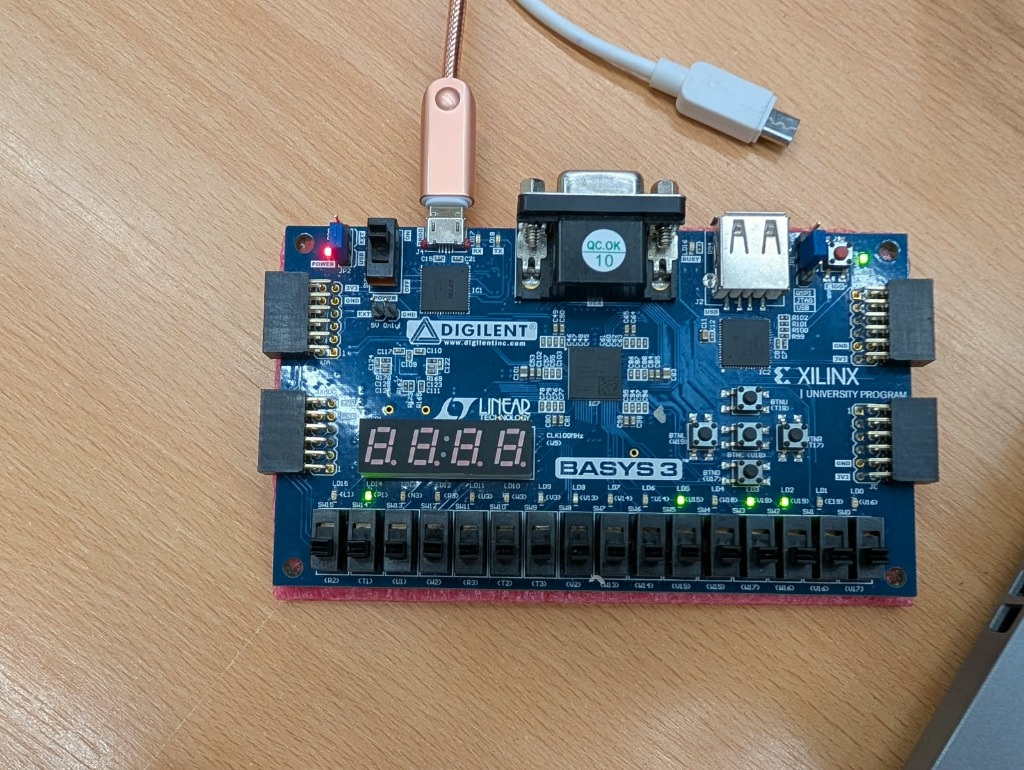
\includegraphics[width=0.52\textwidth, height=3.4cm, keepaspectratio]{basys3_lab.jpg}
\caption{Placa FPGA Digilent Basys 3 en funcionamiento durante los ensayos de laboratorio. Se observa la conexión USB para alimentación y comunicación serie, los interruptores en reposo y los LEDs indicadores de flags reflejando el cálculo de la ALU.}
\label{fig:foto}
\end{figure}
\vspace{-0.6em}

Para validar el enlace se utilizó un script en Python con la librería \texttt{pyserial} (19200-8N1), transmitiendo ternas de bytes con valores conocidos y aleatorios. En cada prueba, el resultado devuelto por la placa coincidió exactamente con el cálculo teórico, confirmando la estabilidad del sobremuestreo y la ausencia de pérdidas de tramas.

% ==============================================================================
\section{Conclusiones}
% ==============================================================================
La integración de la comunicación serie asincrónica resolvió de manera robusta y automática la interacción entre el entorno de desarrollo y la FPGA. El esquema de sobremuestreo $16\times$ garantizó una lectura estable y libre de ruidos en la recepción, mientras que la máquina de estados de \texttt{intf.v} desacopló con éxito la naturaleza secuencial del puerto serie de la naturaleza puramente combinacional de la ALU de 8 bits. Este desarrollo constituye la plataforma de comunicación necesaria sobre la cual se montará la carga de instrucciones en el procesador RISC-V del Trabajo Práctico Final.

\end{document}
